\documentclass[12pt,a4paper]{article}

% ── Packages ──────────────────────────────────────────────
\usepackage[margin=1in]{geometry}
\usepackage{times}
\usepackage{setspace}
\usepackage{graphicx}
\usepackage{titlesec}
\usepackage{enumitem}
\usepackage{hyperref}
\usepackage{xcolor}
\usepackage{fancyhdr}
\usepackage{array}
\usepackage{longtable}
\usepackage{booktabs}
\usepackage{tikz}
\usepackage{float}
\usepackage{caption}
\usepackage{tabularx}
\usepackage{tcolorbox}

\usetikzlibrary{shapes.geometric, arrows.meta, positioning, fit, calc, backgrounds}

\hypersetup{
    colorlinks=true,
    linkcolor=blue!60!black,
    urlcolor=blue!70!black,
    citecolor=black,
}

% ── Spacing & Formatting ─────────────────────────────────
\onehalfspacing
\setlength{\parindent}{0pt}
\setlength{\parskip}{4pt}

\titleformat{\section}{\Large\bfseries}{\thesection.}{0.5em}{}[\vspace{2pt}\titlerule]
\titleformat{\subsection}{\large\bfseries}{\thesubsection}{0.5em}{}
\titleformat{\subsubsection}{\normalsize\bfseries}{\thesubsubsection}{0.5em}{}
\titlespacing*{\section}{0pt}{8pt}{4pt}
\titlespacing*{\subsection}{0pt}{6pt}{2pt}

% ── Header/Footer ────────────────────────────────────────
\pagestyle{fancy}
\fancyhf{}
\lhead{\small\textit{Cloud Computing CIA 1 --- ScholarLens}}
\rfoot{\thepage}
\renewcommand{\headrulewidth}{0.4pt}
\setlength{\headheight}{14pt}
\addtolength{\topmargin}{-2pt}

% ── Column types ─────────────────────────────────────────
\newcolumntype{L}[1]{>{\raggedright\arraybackslash}p{#1}}

% ── GCP highlight box ────────────────────────────────────
\newtcolorbox{gcpbox}{
    colback=green!4, colframe=green!45!black,
    boxrule=0.6pt, arc=2pt, left=6pt, right=6pt, top=3pt, bottom=3pt,
    fontupper=\small, before skip=4pt, after skip=6pt,
}

% ── TikZ styles ──────────────────────────────────────────
\tikzset{
    user/.style={
        ellipse, draw=purple!60!black, fill=purple!8,
        minimum width=2.2cm, minimum height=0.9cm,
        text centered, align=center, text width=1.9cm,
        font=\small\sffamily, line width=0.8pt,
    },
    edge/.style={
        rectangle, draw=blue!60!black, fill=blue!7,
        minimum width=2.6cm, minimum height=0.9cm,
        text centered, align=center, text width=2.6cm,
        rounded corners=3pt, font=\footnotesize\sffamily, line width=0.8pt,
    },
    compute/.style={
        rectangle, draw=teal!70!black, fill=teal!7,
        minimum width=2.6cm, minimum height=0.9cm,
        text centered, align=center, text width=2.6cm,
        rounded corners=3pt, font=\footnotesize\sffamily, line width=0.8pt,
    },
    data/.style={
        rectangle, draw=orange!75!black, fill=orange!8,
        minimum width=2.6cm, minimum height=0.9cm,
        text centered, align=center, text width=2.6cm,
        rounded corners=3pt, font=\footnotesize\sffamily, line width=0.8pt,
    },
    ai/.style={
        rectangle, draw=red!60!black, fill=red!7,
        minimum width=2.6cm, minimum height=0.9cm,
        text centered, align=center, text width=2.6cm,
        rounded corners=3pt, font=\footnotesize\sffamily, line width=0.8pt,
    },
    ext/.style={
        rectangle, draw=gray!70!black, fill=gray!8, dashed,
        minimum width=2.6cm, minimum height=0.9cm,
        text centered, align=center, text width=2.6cm,
        rounded corners=3pt, font=\footnotesize\sffamily, line width=0.8pt,
    },
    flow/.style={-{Stealth[length=2.5mm]}, line width=0.8pt, draw=black!70},
    flowback/.style={-{Stealth[length=2.5mm]}, line width=0.8pt, draw=black!45, dashed},
}

% ══════════════════════════════════════════════════════════
\begin{document}

% ── Title Page ────────────────────────────────────────────
\begin{titlepage}
    \centering
    \vspace*{0.5cm}

    {\large\bfseries CHRIST (Deemed to be University), Bengaluru}\\[4pt]
    {\normalsize Department of Computer Science}\\[1.5cm]

    {\LARGE\bfseries Cloud Computing --- CIA 1}\\[0.4cm]
    {\large Technical Report: Cloud Deployment Plan}\\[0.3cm]
    {\large Semester V Project}\\[1.8cm]

    {\huge\bfseries ScholarLens}\\[0.3cm]
    {\Large Cloud Deployment Plan for a\\ Remote Research Assistant}\\[2.2cm]

    \begin{tabular}{>{\bfseries}r l}
        Student Name: & Aditya Mehta \\[6pt]
        Register No.: & 2440204 \\[6pt]
        Course: & Cloud Computing \\[6pt]
        Assessment: & CIA 1 \\[6pt]
    \end{tabular}

    \vfill
    {\large June 2026}
\end{titlepage}

% ── Abstract ──────────────────────────────────────────────
\begin{center}
    {\Large\bfseries Abstract}
\end{center}

\vspace{0.2cm}

ScholarLens is an offline research literature review agent that ingests PDF
papers, embeds them into a local vector store, and provides hybrid semantic
plus keyword search with Small Language Model (SLM) driven summarisation and
gap analysis. This report presents a cloud deployment plan for extending it
with a \textbf{Remote Research Assistant} --- a feature that connects to a
user's cloud drive, finds and fetches similar papers from the drive and from
external scholarly sources, and indexes them for search. \textbf{Amazon Web
Services (AWS)} is selected as the primary platform; for each service used, the
equivalent \textbf{Google Cloud Platform (GCP)} alternative is highlighted and
consolidated in a comparison table, keeping the design portable. The report
covers the platform choice, the cloud services and the reason for each, the
target architecture and data-flow diagrams, and a deployment strategy.

\vspace{0.3cm}
\hrule
\vspace{0.2cm}
\tableofcontents
\newpage

% ══════════════════════════════════════════════════════════
\section{Introduction}

\subsection{Existing Project Overview}
ScholarLens is built on a modular, domain-driven architecture with a Python
FastAPI backend and a React (Vite) single-page frontend. In its current form
every component runs locally on the user's machine:

\begin{itemize}[leftmargin=2em, nosep]
    \item \textbf{Ingestion} --- PDF parsing, chunking, and metadata
          extraction (PyMuPDF, pdfplumber).
    \item \textbf{Knowledge Base} --- embedding generation with
          Sentence-Transformers and storage in a file-based ChromaDB vector
          database.
    \item \textbf{Search} --- hybrid retrieval combining semantic similarity
          and BM25 keyword search fused with Reciprocal Rank Fusion (RRF).
    \item \textbf{Analysis} --- SLM-powered summarisation, claim extraction,
          and theme clustering using llama.cpp or Ollama.
    \item \textbf{Gap Finder} --- research-gap identification and direction
          suggestion.
\end{itemize}

This offline design guarantees privacy but limits the tool to papers the user
has manually downloaded and to the compute available on a single laptop.

\subsection{The Proposed Cloud Feature: Remote Research Assistant}
The proposed enhancement is a \textbf{Remote Research Assistant} that operates
against the cloud. Given a topic, an existing paper, or the user's whole
library, it will:

\begin{enumerate}[leftmargin=2em, nosep]
    \item \textbf{Connect to a cloud drive} (Google Drive, or an S3 / Cloud
          Storage bucket) belonging to the user and list available PDFs.
    \item \textbf{Find similar papers} by computing semantic similarity at
          scale against a managed vector index, and by querying external
          scholarly APIs (arXiv, Semantic Scholar, CrossRef).
    \item \textbf{Fetch} the selected papers asynchronously, parse and embed
          them, and add them to the searchable knowledge base.
    \item \textbf{Notify} the user when ingestion completes.
\end{enumerate}

This transforms ScholarLens from a single-machine tool into a multi-user,
internet-scale service --- exactly the kind of bursty, storage-heavy,
AI-assisted workload that benefits from elastic, managed cloud infrastructure.

% ══════════════════════════════════════════════════════════
\section{Selected Cloud Platform and Justification}

\textbf{Selected Platform: Amazon Web Services (AWS).} AWS is chosen as the
primary platform for the following reasons:

\begin{itemize}[leftmargin=2em, nosep]
    \item \textbf{Breadth of managed services} --- every component of the
          Remote Research Assistant (container hosting, vector search, managed
          LLMs, object storage, queues, serverless functions) maps to a
          first-party AWS service, minimising operational overhead.
    \item \textbf{Managed vector search} --- Amazon OpenSearch Service
          provides a production-grade k-NN vector index that replaces the
          local ChromaDB store without re-architecting the search logic.
    \item \textbf{Managed foundation models} --- Amazon Bedrock supplies both
          embedding models and generative models, removing the need to
          self-host GPU inference.
    \item \textbf{Mature serverless and eventing} --- Lambda, SQS, and Step
          Functions allow the slow, bursty ``fetch papers'' workload to be
          decoupled from the interactive API.
    \item \textbf{Free-tier and student credits} --- suitable for an academic
          project, with fine-grained, pay-per-use billing.
\end{itemize}

\textbf{Why also consider GCP?} Google Cloud Platform is a strong second
choice and is highlighted throughout this report. Because the headline feature
fetches papers from \emph{Google Drive}, GCP offers tighter native integration
with Google identity and Drive APIs, and its Vertex AI platform provides both
embeddings and the Gemini family of models in a single managed service. To
avoid vendor lock-in, the design is therefore presented as
platform-independent: Section~\ref{sec:services} lists the AWS service and its
GCP equivalent side by side, and Section~\ref{sec:gcp} consolidates the full
mapping.

% ══════════════════════════════════════════════════════════
\section{Cloud Services Used (with GCP Alternatives)}
\label{sec:services}

The application is decomposed into layers. For each layer, this section names
the chosen AWS service, explains \emph{why} it is used, and \textbf{highlights
the GCP alternative} in a shaded box.

\subsection{Storage and Content Delivery --- Amazon S3 + CloudFront}
\textbf{Amazon S3} plays two roles. First, it hosts the built React
single-page app as static files, served globally through the
\textbf{Amazon CloudFront} CDN, which caches assets near users and terminates
HTTPS. Second, it stores the fetched PDF papers, replacing the local
\texttt{data/papers} folder with durable (11 nines), effectively unlimited,
low-cost object storage; lifecycle rules can later archive rarely-read PDFs to
cheaper tiers. Neither role requires a web server to manage.
\begin{gcpbox}
\textbf{GCP alternative:} \textbf{Cloud Storage} behind \textbf{Cloud CDN},
with Nearline/Coldline classes mirroring S3's Infrequent Access / Glacier
tiers --- the same bucket-plus-edge-cache pattern.
\end{gcpbox}

\subsection{Backend Compute and API Entry --- ECS Fargate + API Gateway}
The FastAPI backend is packaged as a container and run on \textbf{Amazon ECS
with the Fargate} launch type. Fargate is serverless: there are no EC2
instances to patch or scale manually, it auto-scales with request load, and we
pay only while containers run. In front of it, \textbf{Amazon API Gateway} is
the single public HTTPS entry point --- routing requests, enforcing throttling
and rate limits, and integrating with authentication so the backend stays off
the public internet.
\begin{gcpbox}
\textbf{GCP alternative:} \textbf{Cloud Run} (runs the same image and scales
to zero when idle) behind \textbf{API Gateway / Cloud Endpoints}.
\end{gcpbox}

\subsection{Authentication --- Amazon Cognito}
\textbf{Amazon Cognito} manages user sign-up/sign-in and brokers the
\emph{Google Drive OAuth} flow, so the assistant can access a user's Drive
without ScholarLens ever storing their Google password. It issues JWT tokens
that API Gateway validates.
\begin{gcpbox}
\textbf{GCP alternative:} \textbf{Firebase Authentication} / \textbf{Identity
Platform}. On GCP this is especially natural because Google sign-in and Drive
access share the same Google identity.
\end{gcpbox}

\subsection{Vector Search --- Amazon OpenSearch Service}
``Find similar papers'' is powered by the k-NN vector index in \textbf{Amazon
OpenSearch Service}. It replaces the local ChromaDB store and performs fast
approximate-nearest-neighbour similarity search across a large, shared
collection of paper embeddings.
\begin{gcpbox}
\textbf{GCP alternative:} \textbf{Vertex AI Vector Search} (formerly Matching
Engine), a purpose-built, highly scalable similarity-search service.
\end{gcpbox}

\subsection{Embeddings and LLM --- Amazon Bedrock}
\textbf{Amazon Bedrock} provides managed foundation models. It generates the
embeddings used for similarity search (e.g.\ Titan Embeddings) and runs the
generative tasks --- summarisation, claim extraction, and gap analysis. This
removes the need to self-host a GPU and the llama.cpp/Ollama runtime that the
offline version required.
\begin{gcpbox}
\textbf{GCP alternative:} \textbf{Vertex AI}, offering text-embedding models
plus the \textbf{Gemini} family for generation through one managed API.
\end{gcpbox}

\subsection{Metadata Store --- Amazon DynamoDB}
Per-paper metadata (title, authors, ingestion status, owning user) is kept in
\textbf{Amazon DynamoDB}, a serverless NoSQL database with single-digit
millisecond reads that scales automatically with the library size.
\begin{gcpbox}
\textbf{GCP alternative:} \textbf{Firestore}, a serverless document database
with the same auto-scaling, pay-per-use model.
\end{gcpbox}

\subsection{Asynchronous Fetch Pipeline --- SQS, Lambda, Step Functions, SNS}
Fetching and processing papers is slow and bursty, so it is handled
out-of-band. Jobs are placed on an \textbf{Amazon SQS} queue and processed by
\textbf{AWS Lambda} workers that scale automatically with the queue depth,
while \textbf{AWS Step Functions} orchestrates the multi-step pipeline
(fetch $\to$ parse $\to$ embed $\to$ index) with built-in retries and error
handling. When the work completes, \textbf{Amazon SNS} notifies the user (by
email or push). The interactive API thus returns immediately and never blocks
on downloads or model inference.
\begin{gcpbox}
\textbf{GCP alternative:} \textbf{Pub/Sub} (queue) + \textbf{Cloud Functions}
(workers) + \textbf{Cloud Workflows} (orchestration) + \textbf{Pub/Sub /
Firebase Cloud Messaging} (notifications).
\end{gcpbox}

\subsection{Supporting Services --- Secrets, Monitoring, Registry}
\textbf{AWS Secrets Manager} stores external API keys and OAuth client
secrets; \textbf{Amazon CloudWatch} and \textbf{AWS CloudTrail} provide logs,
metrics, alarms, and audit trails; \textbf{Amazon ECR} stores the backend
Docker image built by CI/CD.
\begin{gcpbox}
\textbf{GCP alternatives:} \textbf{Secret Manager} (secrets), \textbf{Cloud
Monitoring} + \textbf{Cloud Logging} (observability), and \textbf{Artifact
Registry} (container images).
\end{gcpbox}

% ══════════════════════════════════════════════════════════
\section{System Architecture}

Figure~\ref{fig:arch} shows the target deployment. The interactive path
(browser $\to$ API) is kept fast and synchronous, while the heavy ``fetch
similar papers'' work is pushed onto an asynchronous, event-driven pipeline so
the API never blocks on long downloads or model inference.

\begin{figure}[H]
\centering
\resizebox{\textwidth}{!}{%
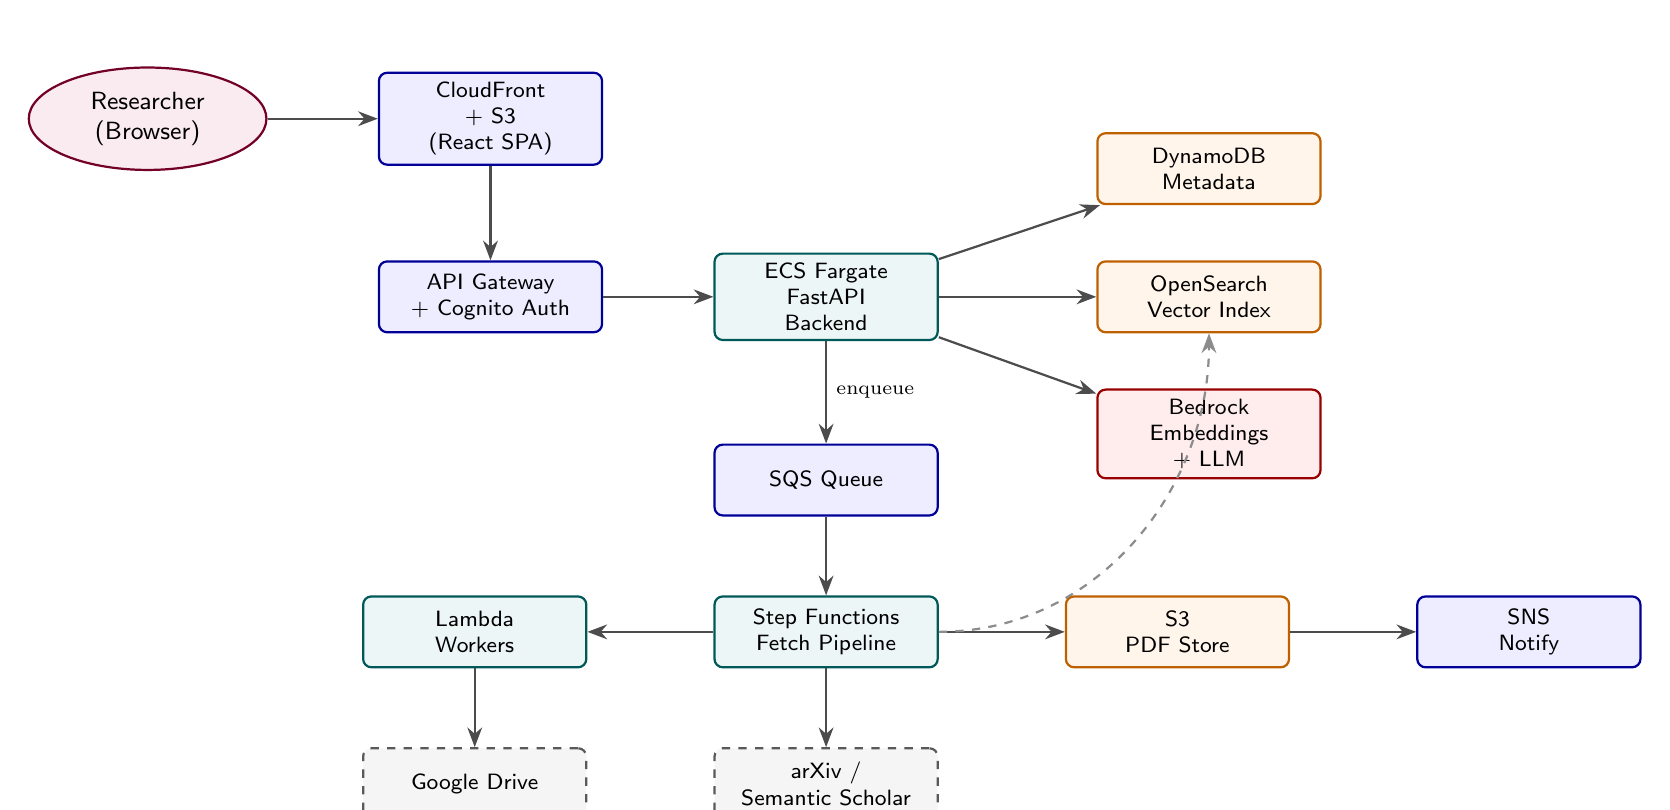
\begin{tikzpicture}[node distance=1.0cm and 1.4cm]

    \node[user] (user) {Researcher\\(Browser)};

    \node[edge, right=of user] (cf) {CloudFront\\+ S3\\(React SPA)};
    \node[edge, below=1.2cm of cf] (apigw) {API Gateway\\+ Cognito Auth};

    \node[compute, right=of apigw] (fargate) {ECS Fargate\\FastAPI\\Backend};

    \node[data, right=2.0cm of fargate] (os) {OpenSearch\\Vector Index};
    \node[data, above=0.7cm of os] (ddb) {DynamoDB\\Metadata};
    \node[ai, below=0.7cm of os] (bedrock) {Bedrock\\Embeddings\\+ LLM};

    \node[edge, below=1.3cm of fargate] (sqs) {SQS Queue};
    \node[compute, below=1.0cm of sqs] (sfn) {Step Functions\\Fetch Pipeline};
    \node[compute, left=1.6cm of sfn] (lambda) {Lambda\\Workers};
    \node[data, right=1.6cm of sfn] (s3) {S3\\PDF Store};

    \node[ext, below=1.0cm of lambda] (drive) {Google Drive};
    \node[ext, below=1.0cm of sfn] (apis) {arXiv /\\Semantic Scholar};
    \node[edge, right=1.6cm of s3] (sns) {SNS\\Notify};

    \draw[flow] (user) -- (cf);
    \draw[flow] (cf) -- (apigw);
    \draw[flow] (apigw) -- (fargate);
    \draw[flow] (fargate) -- (os);
    \draw[flow] (fargate) -- (ddb);
    \draw[flow] (fargate) -- (bedrock);

    \draw[flow] (fargate) -- node[right, font=\scriptsize] {enqueue} (sqs);
    \draw[flow] (sqs) -- (sfn);
    \draw[flow] (sfn) -- (lambda);
    \draw[flow] (sfn) -- (s3);
    \draw[flow] (lambda) -- (drive);
    \draw[flow] (sfn) -- (apis);
    \draw[flow] (s3) -- (sns);

    \draw[flowback] (sfn.east) to[out=0,in=270] (os.south);

\end{tikzpicture}%
}
\caption{Target AWS architecture for the ScholarLens Remote Research
Assistant. Solid arrows: synchronous calls; dashed arrow: the async pipeline
writing results back into the vector index. Each block has a direct GCP
equivalent (see Section~\ref{sec:gcp}).}
\label{fig:arch}
\end{figure}

\subsection{Layer Responsibilities}
\begin{itemize}[leftmargin=2em, nosep]
    \item \textbf{Edge layer} (CloudFront, S3, API Gateway, Cognito) ---
          serves the SPA, terminates TLS, authenticates users, and brokers
          the Google Drive OAuth flow.
    \item \textbf{Compute layer} (ECS Fargate) --- hosts the existing FastAPI
          routes (\texttt{/api/search}, \texttt{/api/documents},
          \texttt{/api/analysis}). Synchronous search and analysis calls fan
          out to OpenSearch, DynamoDB, and Bedrock.
    \item \textbf{Async pipeline} (SQS, Step Functions, Lambda) --- the
          Remote Research Assistant. A fetch request is queued and processed
          out-of-band, so the user is never blocked.
    \item \textbf{Data layer} (S3, OpenSearch, DynamoDB) --- durable PDF
          storage, the vector index, and metadata respectively.
\end{itemize}

% ══════════════════════════════════════════════════════════
\section{Data Flow: Finding and Fetching Similar Papers}

The end-to-end flow for the headline feature is shown in
Figure~\ref{fig:flow}.

\begin{figure}[H]
\centering
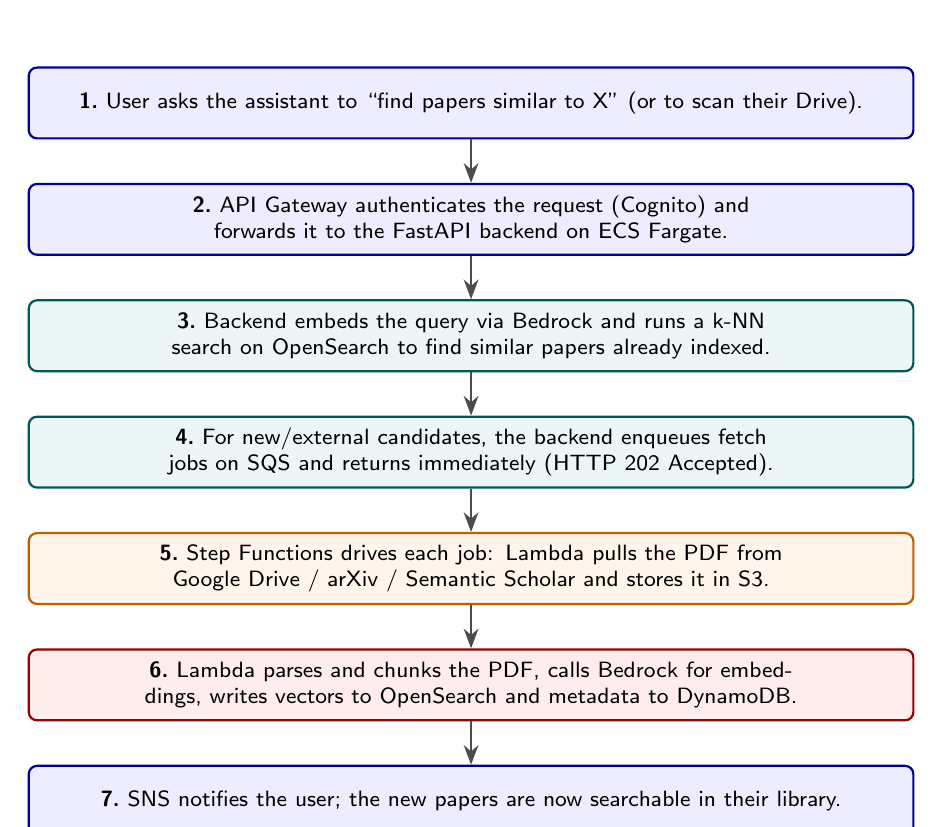
\begin{tikzpicture}[node distance=0.55cm, font=\footnotesize\sffamily]
    \node[edge, text width=11cm] (s1)
        {\textbf{1.}~User asks the assistant to ``find papers similar to X''
         (or to scan their Drive).};
    \node[edge, text width=11cm, below=of s1] (s2)
        {\textbf{2.}~API Gateway authenticates the request (Cognito) and
         forwards it to the FastAPI backend on ECS Fargate.};
    \node[compute, text width=11cm, below=of s2] (s3)
        {\textbf{3.}~Backend embeds the query via Bedrock and runs a k-NN
         search on OpenSearch to find similar papers already indexed.};
    \node[compute, text width=11cm, below=of s3] (s4)
        {\textbf{4.}~For new/external candidates, the backend enqueues fetch
         jobs on SQS and returns immediately (HTTP 202 Accepted).};
    \node[data, text width=11cm, below=of s4] (s5)
        {\textbf{5.}~Step Functions drives each job: Lambda pulls the PDF from
         Google Drive / arXiv / Semantic Scholar and stores it in S3.};
    \node[ai, text width=11cm, below=of s5] (s6)
        {\textbf{6.}~Lambda parses and chunks the PDF, calls Bedrock for
         embeddings, writes vectors to OpenSearch and metadata to DynamoDB.};
    \node[edge, text width=11cm, below=of s6] (s7)
        {\textbf{7.}~SNS notifies the user; the new papers are now searchable
         in their library.};

    \draw[flow] (s1) -- (s2);
    \draw[flow] (s2) -- (s3);
    \draw[flow] (s3) -- (s4);
    \draw[flow] (s4) -- (s5);
    \draw[flow] (s5) -- (s6);
    \draw[flow] (s6) -- (s7);
\end{tikzpicture}
\caption{Data flow for discovering, fetching, and indexing similar papers.}
\label{fig:flow}
\end{figure}

The key design decision is the \textbf{synchronous/asynchronous split}:
similarity search against already-indexed papers returns instantly
(steps 1--3), while fetching brand-new papers from the drive or the open web
(steps 4--7) happens in the background. This keeps the UI responsive even when
dozens of large PDFs are being downloaded and embedded. On GCP the same flow
runs with Cloud Run, Vertex AI, Pub/Sub, Cloud Functions, and Cloud Workflows
in place of the AWS services.

% ══════════════════════════════════════════════════════════
\section{AWS to GCP Service Mapping}
\label{sec:gcp}

Table~\ref{tab:gcp} consolidates the side-by-side mapping. The architecture and
data flow are unchanged across providers; only the managed services differ,
which keeps ScholarLens portable and avoids lock-in to a single vendor.

\renewcommand{\arraystretch}{1.3}
\begingroup
\singlespacing
\begin{longtable}{L{3.7cm} L{4.2cm} L{4.6cm}}
\caption{AWS service used in ScholarLens and its GCP alternative.}
\label{tab:gcp}\\
\toprule
\textbf{Function} & \textbf{AWS (chosen)} & \textbf{GCP alternative} \\
\midrule
\endfirsthead
\multicolumn{3}{l}{\small\itshape (continued from previous page)}\\
\toprule
\textbf{Function} & \textbf{AWS (chosen)} & \textbf{GCP alternative} \\
\midrule
\endhead
\bottomrule
\endfoot
Frontend + CDN      & S3 + CloudFront        & Cloud Storage + Cloud CDN \\
Object storage      & S3                     & Cloud Storage \\
API gateway         & API Gateway            & API Gateway / Cloud Endpoints \\
Container compute    & ECS on Fargate         & Cloud Run \\
Authentication      & Cognito                & Firebase Auth / Identity Platform \\
Vector search       & OpenSearch (k-NN)      & Vertex AI Vector Search \\
Embeddings + LLM    & Bedrock (Titan)        & Vertex AI (Gemini / text-embeddings) \\
Metadata store      & DynamoDB               & Firestore \\
Async functions     & Lambda                 & Cloud Functions \\
Message queue       & SQS                    & Pub/Sub \\
Orchestration       & Step Functions         & Cloud Workflows \\
Notifications       & SNS                    & Pub/Sub / Firebase Cloud Messaging \\
Secrets             & Secrets Manager        & Secret Manager \\
Observability       & CloudWatch + CloudTrail& Cloud Monitoring + Cloud Logging \\
Container registry  & ECR                    & Artifact Registry \\
\end{longtable}
\endgroup
\renewcommand{\arraystretch}{1.0}

\textbf{When would GCP be preferable?} Because the Remote Research Assistant
reads from \emph{Google Drive}, a GCP deployment benefits from native Google
identity integration (one OAuth consent covers sign-in and Drive access) and
from Vertex AI bundling embeddings and the Gemini generative models behind a
single API. AWS is chosen here for its slightly broader free tier and the
maturity of its serverless eventing stack, but the application is deliberately
written to run on either.

% ══════════════════════════════════════════════════════════
\section{Deployment Strategy}

\subsection{Containerisation}
The FastAPI backend is packaged as a Docker image and pushed to Amazon ECR
(Artifact Registry on GCP). The React frontend is built
(\texttt{npm run build}) into static assets and uploaded to S3 (Cloud Storage
on GCP). Using a container means the same image runs identically in local
development, staging, and production.

\subsection{Infrastructure as Code (IaC)}
All cloud resources --- network, container service, vector index, databases,
buckets, functions, and IAM roles --- are defined declaratively with
\textbf{Terraform}, which supports both AWS and GCP. This makes the environment
reproducible, version-controlled, and easy to tear down, which matters for an
academic project running on limited credits.

\subsection{CI/CD Pipeline}
A pipeline (GitHub Actions, or AWS CodePipeline / GCP Cloud Build) automates
delivery:
\begin{enumerate}[leftmargin=2em, nosep]
    \item \textbf{Build} --- run backend tests, build the Docker image, build
          the React bundle.
    \item \textbf{Publish} --- push the image to the registry; sync the
          frontend bundle to object storage and invalidate the CDN cache.
    \item \textbf{Deploy} --- apply Terraform and trigger a rolling deployment
          (ECS Fargate / Cloud Run) with health-check-based rollback.
\end{enumerate}

\subsection{Scalability}
\begin{itemize}[leftmargin=2em, nosep]
    \item ECS Fargate / Cloud Run auto-scale backend tasks on CPU and request
          metrics.
    \item Lambda / Cloud Functions scale automatically with the queue
          backlog, absorbing sudden bursts of fetch jobs.
    \item OpenSearch / Vertex AI Vector Search and DynamoDB / Firestore scale
          by capacity mode; CloudFront / Cloud CDN absorb frontend traffic at
          the edge.
\end{itemize}

\subsection{Security}
\begin{itemize}[leftmargin=2em, nosep]
    \item Least-privilege IAM roles per service; no long-lived credentials in
          code.
    \item Secrets held in Secrets Manager / Secret Manager.
    \item Encryption at rest (S3, DynamoDB, OpenSearch / their GCP
          equivalents) and in transit (TLS everywhere).
    \item Cognito / Firebase JWTs authorise API calls; the backend runs in
          private subnets with no direct public exposure.
\end{itemize}

\subsection{Cost Optimisation}
A serverless-first design (Fargate, Lambda, S3, DynamoDB on-demand --- or
Cloud Run, Cloud Functions, Cloud Storage, Firestore) means the project pays
only for actual usage and effectively nothing while idle. Object-storage
lifecycle rules archive rarely-read PDFs, and Bedrock / Vertex AI bill per
token rather than per provisioned GPU hour.

% ══════════════════════════════════════════════════════════
\section{Conclusion}

This report presented a cloud deployment plan for extending ScholarLens with a
Remote Research Assistant capable of discovering and fetching similar papers
from a user's cloud drive and from external scholarly sources. AWS was selected
as the primary platform because its managed services --- ECS Fargate for
compute, OpenSearch for vector search, Bedrock for embeddings and language
models, and an SQS/Lambda/Step Functions pipeline for asynchronous fetching ---
map cleanly onto the application's existing domain-driven structure. For every
service, the equivalent GCP offering (Cloud Run, Vertex AI, Pub/Sub, Cloud
Functions, Cloud Workflows, and others) was highlighted, leaving ScholarLens
portable across both providers. The synchronous/asynchronous split keeps
interactive search fast while offloading slow fetch-and-index work to an
elastic, event-driven backend, and a serverless-first, infrastructure-as-code
deployment with CI/CD delivers a reproducible, secure, and cost-efficient
system.

\end{document}
